\section{Example}
\label{sec:example}

TeMAPI includes three major steps in detecting behavioral differences among API elements described in mapping relations. We use JLCA (a Java-to-C\# translation tool) as an example translation tool, and the \CodeIn{java.io.ByteArrayInputStream} class in Java as an example API element to illustrate these three steps.

%----------------------------------------------------

\textbf{Translating Synthesized Wrappers.} TeMAPI first synthesizes Java wrapper methods for public methods and fields of the example class. TeMAPI next uses JLCA to translate the wrapper methods to C\#. TeMAPI next compiles the translated wrapper methods, and compares source code of the synthesized wrapper methods with the compilation-error-free translated wrapper methods to extract translatable API elements of the example class. In particular, our example class in Java has five fields, two constructors, and eight methods besides inherited ones\footnote{\url{http://download.oracle.com/javase/6/docs/api/java/io/ByteArrayInputStream.html}}. A class can have more than one constructor, and a translation tool may not translate all its constructors. Therefore, to address this issue, TeMAPI includes different constructors in its synthesized wrapper methods instead of simply pushing the receiver object as a parameter of wrapper methods. For example, TeMAPI first identifies \CodeIn{ByteArrayInputStream(byte[])} constructor as translatable, and synthesizes the wrapper method for the \CodeIn{skip(long)} method as follows:

\begin{CodeOut}%\vspace*{-1.5ex}
\begin{alltt}
public long testskip24nm(long m0, byte c0[])\{
  ByteArrayInputStream obj = new ByteArrayInputStream(c0);
  return obj.skip(m0);
\}
\end{alltt}
\end{CodeOut}%\vspace*{-1ex}

TeMAPI next uses JLCA to translate synthesized wrapper methods from Java to C\#. A translation tool typically cannot include mapping relations for all the API elements between two languages, so translated wrapper methods can have compilation errors. TeMAPI parses translated wrapper methods and filters out all methods with compilation errors. For example, below is the translated \CodeIn{testskip24nm} method in C\#:

\begin{CodeOut}%\vspace*{-1.5ex}
\begin{alltt}
public virtual long testskip24nm(long m0, sbyte[] c0)\{
  MemoryStream obj = new MemoryStream(
                    SupportClass.ToByteArray(c0));
  MemoryStream temp_BufferedStream = obj;
  Int64 temp_Int64 = temp_BufferedStream.Position;
  temp_Int64 = temp_BufferedStream.Seek(m0,
       System.IO.SeekOrigin.Current) - temp_Int64;
  return temp_Int64;
\}
\end{alltt}
\end{CodeOut}%\vspace*{-1ex}

TeMAPI does not remove this method, since it does not result in compilation errors.


\textbf{Generating C\# Test Cases for Testing Java Code.} A major advantage of our synthesized wrapper method is that the synthesized wrapper method and the translated wrapper method have the same numbers/orders of inputs and types of inputs are mapped, irrespective of method calls within the wrapper method. Therefore, TeMAPI detects behavioral differences between mapped API elements by generating test cases on one language version of wrapper methods and applying those test cases on the other language version. In particular, TeMAPI extends Pex~\cite{tillmann2008pex} to generate test cases for each remaining C\# wrapper method. For the example class, Pex attempts to explore all feasible paths among method calls within the wrapper methods and generates inputs and outputs that exercise various paths. Based on the inputs and output generated for each path, TeMAPI generates a Java test case to check whether the original wrapper method return the same values as the translated one. For example, TeMAPI generates the following Java test case based on inputs generated by Pex for one feasible path (in the C\# wrapper method) that throws exceptions (see Section~\ref{sec:approach:single} for details of generating Java test cases).

\begin{CodeOut}%\vspace*{-1.5ex}
\begin{alltt}
public void testskip24nm36()\{
  try\{
     Test_java_io_ByteArrayInputStream obj =
        new Test_java_io_ByteArrayInputStream();
     long m0 = java.lang.Long.valueOf(
                  "2147483648").longValue();
     byte[] c0 = new byte[0];
     obj.testskip24nm(m0,c0);
     Assert.assertTrue(false);
  \}catch(java.lang.Exception e)\{
     Assert.assertTrue(true);
  \}
\}
\end{alltt}
\end{CodeOut}%\vspace*{-2ex}

This Java test case fails, since given the preceding inputs, the \CodeIn{skip (long)} method in Java does not throw any exceptions, instead the translated C\# code does. Thus, TeMAPI detects a behavioral difference between the \CodeIn{skip(long)} method in Java and its translated C\# API elements by JLCA.

%-----------------------------------
\textbf{Generating Java Test Cases for Testing C\# Code.} As shown by Thummalapenta \emph{et al.}~\cite{thummalapenta09:mseqgen}, Pex cannot effectively generate sequences. To address this issue, TeMAPI extends Randoop~\cite{pacheco2007feedback} for testing Java code to generate invocation sequences. TeMAPI does not generate invocation sequences from wrappers directly, since each wrapper method includes a fixed simple invocation sequence. Instead, TeMAPI uses translatable API methods in Step 1, and limits the scope of Randoop to those methods while generating invocation sequences. For example, a generated Java test case is as follows:

\begin{CodeOut}%\vspace*{-1.5ex}
\begin{alltt}
public void test413() throws Throwable\{
  ...
  ByteArrayInputStream var2=new ByteArrayInputStream(...);
  var2.close();
  int var5=var2.available();
  assertTrue(var5 == 1);
\}
\end{alltt}
\end{CodeOut}%\vspace*{-1ex}


The test case gets passed, since Java allows access to the stream even if the stream is closed. TeMAPI next uses JLCA to translate the generated Java test case from Java to C\#. Since the Java test case uses only translatable API elements, JLCA translates the test case to a C\# test case as follows:

\begin{CodeOut}%\vspace*{-1.5ex}
\begin{alltt}
public void test413() throws Throwable\{
  ...
  MemoryStream var2 = new MemoryStream(...);
  var2.close();
  long available = var2.Length - var2.Position;
  int var5 = (int) available;
  AssertTrue(var5 == 1);
\}
\end{alltt}
\end{CodeOut}%\vspace*{-1ex}

In contrast to the Java test case, the C\# test case gets failed since C\# does not allow such access to the stream and throws \CodeIn{ObjectDis\\posedException}. TeMAPI thus detects a behavioral difference with invocation sequences.

This example motivates our basic idea of generating test cases in one language and translating those test cases to another language for detecting differences among API mapping relations. %We next present details of our approach.

%\begin{figure}[t]
%\centering %\hfill
%\includegraphics[scale=0.95,clip]{figure/sample.eps}\vspace*{-3ex}
% \caption{\label{fig:example}API mapping}\vspace*{-4ex}
%\end{figure}

%Based on the mapping relations, a translation tool can migrate the
%preceding code snippet automatically. To learn the mapping
%relations,
%
%%\begin{figure}[t]
%%\centering
%%\includegraphics[scale=0.86,clip]{figure/openfile.eps}\vspace*{-1.5ex}
%% \caption
%%{\label{fig:openfile}Aligned wrapper}\vspace*{-2ex}
%%\end{figure}
%
%In this section, we illustrate the main steps of MAM to
%mine the API mapping in Java for \CodeIn{System.IO.Directory.
%Exists()} in C\# from the HypoLog
%project\footnote{\url{http://sourceforge.net/projects/twlog/}}.
%
%The first step of MAM is to align classes and methods of
%wrapper by names. This step finds class pairs and method pairs
%that implement similar functionalities, and each pair may use
%API mapping since it implements a similar functionality. Our
%approach chooses names to align classes and methods because these
%classes and methods are from the same project. In this example, our
%approach aligns the two methods as shown in
%Figure~\ref{fig:openfile} because the two method have similar names
%and their declaring classes also have similar names (see
%Section~\ref{sec:approach:alignclientcode} for details).
%
%The second step of MAM is to mine mapping relations of API
%classes based on the names of corresponding fields, parameters,
%returned types, and local variables. This step also relies on names
%for the same consideration of the first step. For example, our
%approach maps the two parameters with the same name as shown by the
%red arrow of Figure~\ref{fig:openfile}. From the types of the two
%parameters, MAM mines the mapping relation between two API
%classes: \CodeIn{System.String} $\leftrightarrow$
%\CodeIn{java.lang.String} (see
%Section~\ref{sec:approach:mappingtypes} for details).
%
%
%The final step of MAM is to mine mapping relations of API
%methods. Besides the factors listed in
%Section~\ref{sec:introduction}, another factor is that API calls in
%wrapper are often not carefully aligned. To deal with those
%challenges, MAM first builds an API Transformation Graph
%(ATG) for each method. After that, MAM compares built
%graphs to mine mapping relations of API methods (see
%Section~\ref{sec:approach:mappingtypes} and
%Figure~\ref{fig:approach1} for details). Figure~\ref{fig:example}
%shows the mined mapping relation between
%\CodeIn{System.IO.Directory.Exists()} and its API mapping in
%Java.
